\documentclass{article}
\usepackage{tikz}
\usepackage{CJKutf8}
\usepackage{amsmath}
\usepackage{amsthm}
\begin{document}
\begin{CJK}{UTF8}{gbsn}
  \newtheorem*{Exercise}{习题}
  \huge
\begin{Exercise}[p314-4]
  有向图$D$的图解如下图所示:
  
\large
  \centering
  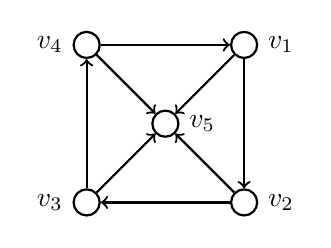
\begin{tikzpicture}[auto,
    specification/.style ={circle, draw, thick}]
   \node[specification] (A) [label=0:$v_1$] at (1,1)  {};
   \node[specification] (B) [label=0:$v_2$] at (1,-1)  {};
   \node[specification] (C) [label=180:$v_3$] at (-1,-1)  {};
   \node[specification] (D) [label=180:$v_4$] at (-1,1)  {};
   \node[specification] (E) [label=0:$v_5$] at (0,0)  {};
   
   \draw[thick, ->] (A) to  (B);
   \draw[thick, ->] (B) to  (C);
   \draw[thick, ->] (C) to  (D);
   \draw[thick, ->] (D) to  (A);
   \draw[thick, ->] (A) to  (E);
   \draw[thick, ->] (B) to  (E);
   \draw[thick, ->] (C) to  (E);
   \draw[thick, ->] (D) to  (E);   
 \end{tikzpicture}\hspace{1cm}\\
 D
\flushleft\huge
求从顶点$v_2$到其余每个顶点的长$\leq 4$的所有有向通道的条数。 
\end{Exercise}

\end{CJK}
\end{document}


%%% Local Variables:
%%% mode: latex
%%% TeX-master: t
%%% End:
